\chapter{Conclusions}

\section{Summary}

The implementation can successfully generate parity data and repair file corruption using Reed-Solomon codes.

The file metadata is currently not protected from corruption.
This can be addressed by adding meta-parity blocks among the parity blocks.
Although the metadata is generally small, this is a significant flaw in the current implementation.

Only a single data file and parity file are supported. Multiple input files and single-file archives would be a useful feature to add.
This would require significal re-architecting of the program's I/O in order to read and write blocks to arbitrary files in arbitrary folder structures.
The file header of the parity file would need to be extended to include relative paths to the data files.
Single-file archives would be less difficult to add.

\pagebreak

\section{Figures}

% TODO: move this section to an annex

As a final note, and to visually demonstrate some limitations of this error correction scheme,
the following figures show the use of Reed-Solomon codes to repair bitmap images.

Figure B is impossible to repair, yet figure A has more errors.
This is because the errors in figure A are contiguous - they are burst errors - so they affect less blocks.

Figure C is the recovered image from figure A.

See the script \texttt{generate\_figures.py} for how these images were generated.

\begin{figure}[H]
    \centering
    \begin{subcaptionbox}{A bitmap image with repairable errors.}
        {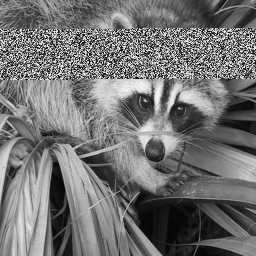
\includegraphics[width=0.3\textwidth]{face_2.png}}
    \end{subcaptionbox}
    \hfill
    \begin{subcaptionbox}{A bitmap image with irreparable errors.}
        {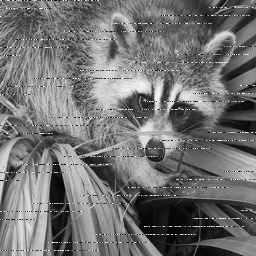
\includegraphics[width=0.3\textwidth]{face_3.png}}
    \end{subcaptionbox}
    \hfill
    \begin{subcaptionbox}{Figure A, repaired.}
        {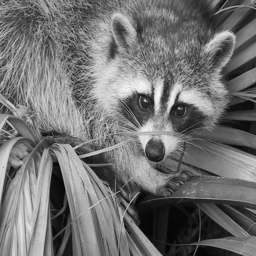
\includegraphics[width=0.3\textwidth]{face_2_repaired.png}}
    \end{subcaptionbox}
    
    \caption{Image source: \texttt{scipy.datasets.face}.}
\end{figure}
